\documentclass{beamer}
\usetheme{metropolis} 

\usepackage{xcolor}
\usepackage[utf8]{inputenc}
\usepackage{hyphenat}
\usepackage[russian,english]{babel}          % Use metropolis theme

% Указывайте все новые термины в \termdef команде. А уже известные ранее или из других курсов в \term
\newcommand{\termdef}[1]{\textbf{\textit{#1}}}
\newcommand{\term}{\textit}
% Диалог с аудиторией.
\newcommand{\auditorium}[1]{\color{red}{\textbf{#1}}}
% \setbeamercolor{auditorium}{fg=red}

\title{Лекция 2. Экспертные системы. Основные параметры качества.}
% \date{\today}
\date{9 сентября 2019}
\author{Павел Владимирович Слипенчук}
\institute{Москва, МГТУ им.Бауманка,\\ каф.ИУ-8, КИБ}
% \titlegraphic{\includegraphics[width=2cm]{logo_ur.jpg}}
\titlegraphic{\small \href{https://github.com/kib-courses/dsis}{Data Science для решения задач информационной безопасности}}

\begin{document}
  \maketitle
    
  \begin{frame}{План лекции}
    \begin{enumerate}
	\item \nameref{section:classification_defs}
	\item второе
	\end{enumerate}
 \end{frame}
    
  \section{Признак. Вектор признаков Классы. Обучающая и тестовая выборки. Задача классификации, классификатор(оценщик)}\label{section:classification_defs}
  
  \begin{frame}
    \termdef{Признак} ($x_i$)-- определенное значение. Категориальное, сравнимое, или числовое: целочисленное, булевое, или дробное.
    
    \termdef{Вектор признаков} ($\bold x = (x_1, x_2, ... x_n)$) -- вектор, каждое значение которого является \term{признаком}. 
  	
  	\termdef{Класс} (метка) -- значение (как правило целочисленное), присваиваемое какому-либо
  	вектору признаков
  	
  	\auditorium{А в чем физический смысл?}
  \end{frame}
  
  
  \begin{frame}{Классификация}
    \termdef{Классификация} -- это одна из задач \term{машинного обучения}, для которой каждому
    вектору признаков $\bold x = (x_1, x_2, ..., x_n)$ присваивается какой-либо \term{класс}.
    \newline
    \begin{center}
    	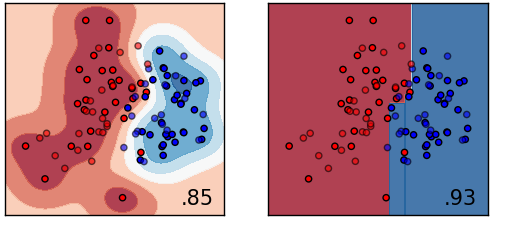
\includegraphics[width=8cm]{pic/classification_example.png}\centering
    \end{center}
	
  \end{frame}

\end{document}